\documentclass[11pt]{article}
\usepackage[utf8]{inputenc}	% Para caracteres en español
\usepackage{amsmath,amsthm,amsfonts,amssymb,amscd}
\usepackage{multirow,booktabs}
\usepackage[table]{xcolor}
\usepackage{fullpage}
\usepackage{lastpage}
\usepackage{enumitem}
\usepackage{fancyhdr}
\usepackage{mathrsfs}
\usepackage{wrapfig}
\usepackage{setspace}
\usepackage{calc}
\usepackage{multicol}
\usepackage{cancel}
\usepackage{float}
\usepackage{physics}
\usepackage[retainorgcmds]{IEEEtrantools}
\usepackage[margin=1cm]{geometry}
\usepackage{amsmath}
\newlength{\tabcont}
\setlength{\headheight}{14pt}
\setlength{\parindent}{0.0in}
\setlength{\parskip}{0.05in}
\usepackage{empheq}
\usepackage{framed}
\usepackage[most]{tcolorbox}
\usepackage{xcolor}
\usepackage[version=3]{mhchem}
\usepackage[english]{babel}
\usepackage[utf8]{inputenc}
\usepackage{graphicx}
\usepackage[colorinlistoftodos]{todonotes}
\usepackage{mdframed}

\colorlet{shadecolor}{orange!15}
\parindent 0in
\parskip 12pt
\geometry{margin=1in, headsep=0.45in}
\theoremstyle{definition}
\newtheorem{defn}{Definition}
\newtheorem{reg}{Rule}
\newtheorem{exer}{Exercise}
\newtheorem{note}{Note}
\begin{document}
\setcounter{section}{2}
%\setcounter{subsection}{}
\title{Problem Set 11}

%==============================================================
%\thispagestyle{empty}
\pagestyle{fancy}
\fancyhf{}
\rhead{Physics 180}
\chead{Problem Set 11}
\lhead{Olyn D. Desabelle}
\rfoot{Page \thepage}

\begin{center}
{\LARGE \bf Problem Set 11}\\
%{\large Physics 180}\\
%Olyn D. Desabelle
\end{center}

%==============================================================
\begin{figure}[H]
    \centering
    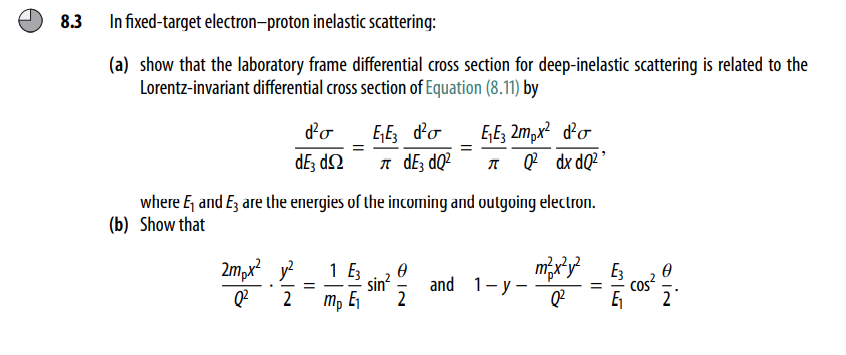
\includegraphics[scale = 0.5]{8.3a.png}
    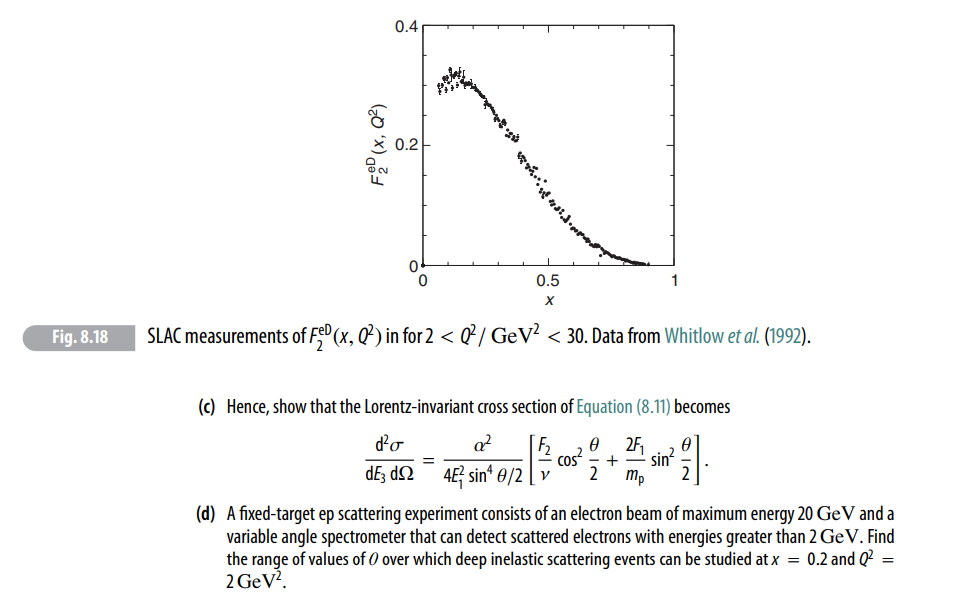
\includegraphics[scale = 0.5]{8.3b.png}
\end{figure}

\underline{a)}

Equation (8.11) gives:

\begin{align}
    \frac{d^2\sigma}{dxdQ^2}
    =
    \frac{4\pi\alpha^2}{Q^4}
    \left[
        \left(
            1 - y - \frac{m_p^2y^2}{Q^2}
        \right)
        \frac{F_2(x,Q^2)}{x}
        +
        y^2F_1(xQ^2)
    \right]
\end{align}

for a differential cross-section, we may express $d\Omega$ as:

\begin{align}
    d\Omega = 2\pi d \cos\theta
\end{align}

in order to express this in terms of $Q^2$, we use the approximation of $Q^2$:

\begin{align}
    Q^2 &\approx 2E_1E_3(1-\cos\theta)\\
    \absolutevalue{\frac{dQ^2}{d\cos\theta}} &= 2E_1E_3 
\end{align}

thus we have:

\begin{align}
    \frac{d^2\sigma}{dE_3d\Omega}
    &=
    \frac{d^2\sigma}{dE_3(2\pi d\cos\theta)}\\
    &= \frac{1}{2\pi}\frac{d^2\sigma}{dE_3\left(\frac{dQ^2}{2E_1E_3}\right)}
\end{align}

\begin{equation}
\boxed{
    \frac{d^2\sigma}{dE_3d\Omega}
    =
    \frac{E_1E_3}{\pi}\frac{d^2\sigma}{dE_3dQ^2}
}
\end{equation}

we may rewrite $dE_3$ in terms of $x$ by noting:

\begin{align}
    x &= \frac{Q^2}{2m_pv}\\
    v &= \frac{Q^2}{2m_px}\\
    v &= E_1-E_3\\
    \frac{dv}{dE_3} &= -1\\
    \frac{dv}{dx} &= -\frac{Q^2}{2m_px^2}\\
\end{align}

we rewrite the RHS of the equation obtained earlier as:

\begin{align}
    \frac{E_1E_3}{\pi}\frac{d^2\sigma}{dE_3dQ^2}
    &=
    -\frac{E_1E_3}{\pi}
    \frac{d^2\sigma}{dvdQ^2}\\
    &=
    \frac{E_1E_3}{\pi}
    \frac{2m_px^2}{Q^2}\frac{d^2\sigma}{dxdQ^2}
\end{align}

equating this to the LHS, we get:

\begin{equation}\label{part a final}
\boxed{
    \frac{d^2\sigma}{dE_3d\Omega}
    =
    \frac{E_1E_3}{\pi}
    \frac{2m_px^2}{Q^2}\frac{d^2\sigma}{dxdQ^2}
}
\end{equation}
%==============================================================
\newpage
\underline{b)}

We first aim to show that:

\begin{align}\label{prove b1}
    \frac{2m_px^2}{Q^2}\cdot \frac{y^2}{2} = \frac{1}{m_p}\frac{E_3}{E_1}\sin^2\frac{\theta}{2}
\end{align}

We note the approximation for $Q^2$ given negligible electron mass:

\begin{align}
    Q^2 \approx 2E_1E_3(1-\cos\theta) &= 4E_1E_3\sin^2\frac{\theta}{2}\\
\end{align}

Rearranging terms, we have:

\begin{align}
    E_3\sin^2\frac{\theta}{2} &= \frac{Q^2}{4E_1}\\
\end{align}

We may divide both sides by $E_1$ to have:

\begin{align}\label{eq 1}
    \frac{E_3}{E_1}\sin^2\frac{\theta}{2} &= \frac{Q^2}{4E_1^2}\\
\end{align}

We next note that in the frame where the proton is at rest (meaning $p_2 = (m_p,0,0,0)$), the inelasticity $y$ may be written as:

\begin{align}
    y &= \frac{m_p(E_1-E_3)}{m_pE_1} = 1-\frac{E_3}{E_1}\\
    1-y &= \frac{E_3}{E_1}
\end{align}

and $v$ may be written as:

\begin{align}
    v &= \frac{p_2 \cdot q}{m_p} = E_1-E_3
\end{align}

the relationship between $y$ and $v$ may then be described by:

\begin{align}
    y &= \frac{v}{E_1}
\end{align}

%Thus we may rewrite Equation \ref{eq 1} as:

%\begin{align}\label{eq 2}
%    \frac{E_3}{E_1}\sin^2\frac{\theta}{2} &= \frac{Q^2y^2}{4v^2}\\
%\end{align}

With the relations between $Q^2$ and $x$ given in Equation 8.6 of Thomson, we have:

\begin{align}
    x &= \frac{Q^2}{2m_pv}\\
    %x &= \frac{Q^2}{2m_p(E_1-E_3)}
\end{align}

using these on the LHS of Equation \ref{prove b1}, we get:

\begin{align}
    \frac{2m_px^2}{Q^2}\cdot \frac{y^2}{2}
    &= \frac{2m_p}{Q^2}\left(\frac{Q^2}{2m_pv}\right)^2\cdot\frac{y^2}{2}\\
    &= \frac{Q^2}{2m_pv^2} \cdot \frac{y^2}{2}\\
    &= \frac{Q^2}{4m_p}  \left(\frac{1}{E_1^2}\right) \\
    &= \frac{1}{4m_p} \left(4E_1E_3\sin^2\frac{\theta}{2}\right)  \left(\frac{1}{E_1^2}\right) \\
    %&= 2m_p \left( \frac{1}{4m_p^2(E_1-E_3)^2} \right)
    %\left( Q^24E_1E_3\sin^2\frac{\theta}{2} \right) 
    %%\left( \frac{1}{4E_1E_3\sin^2\frac{\theta}{2} } \right) 
    %\cdot \frac{(E_1-E_3)}{2E_1}\\
    %&= 2m_p \left( \frac{1}{m_p^2(E_1-E_3)} \right)
    %\left( E_1E_3\sin^2\frac{\theta}{2} \right) 
    %\left( \frac{1}{4E_1E_3\sin^2\frac{\theta}{2} } \right) 
    %\cdot \frac{1}{2E_1}\\
\end{align}

%===

%using this to replace $v$ in Equation \ref{eq 2}, we get:

%\begin{align}\label{eq 3}
%    \frac{E_3}{E_1}\sin^2\frac{\theta}{2} &= \frac{Q^2y^2}{4}\frac{4m_p^2x^2}{Q^2}\\
%\end{align}

%we may divide both sides by $m_p$ and get:

%\begin{align}
%    \frac{1}{m_p}\frac{E_3}{E_1}\sin^2\frac{\theta}{2} &= m_px^2y^2\\
%\end{align}

%switching sides and multiplying the LHS by 1 gives:

%\begin{align}
%    m_px^2y^2 \left(\frac{2}{2}\right) &= \frac{1}{m_p}\frac{E_3}{E_1}\sin^2\frac{\theta}{2} \\
%\end{align}

Finally, we get:

\begin{equation}\label{part b initial}
\boxed{
    \frac{2m_px^2}{Q^2} \cdot \frac{y^2}{2} = \frac{1}{m_p}\frac{E_3}{E_1}\sin^2\frac{\theta}{2} 
}
\end{equation}

The next equation we prove is:

\begin{align}
    1-y-\frac{m_p^2x^2y^2}{Q^2} = \frac{E_3}{E_1}\cos^2\frac{\theta}{2}
\end{align}

expanding the RHS, we get:

\begin{align}
    \frac{E_3}{E_1}\cos^2\frac{\theta}{2}
    &=
    \frac{E_3}{E_1}\left[1 - \sin^2\frac{\theta}{2}\right]\\
    &=\left[\frac{E_3}{E_1} - \frac{E_3}{E_1}\sin^2\frac{\theta}{2}\right]\frac{m_p}{m_p}\\
    &=\frac{m_pE_3}{m_pE_1} - \frac{m_p}{m_p}\frac{E_3}{E_1}\sin^2\frac{\theta}{2}\\
    &=\frac{E_3}{E_1} - \left(\frac{m_p^2x^2y^2}{Q^2}\right)\\
\end{align}

where in the last step we used the recently obtained Equation \ref{part b initial}. This leads us to:

\begin{equation}\label{part b final}
\boxed{
    1-y-\frac{m_p^2x^2y^2}{Q^2} = \frac{E_3}{E_1}\cos^2\frac{\theta}{2}
}
\end{equation}

%==============================================================
\newpage
\underline{c)}

Equation (8.11) gives:

\begin{align}
    \frac{d^2\sigma}{dxdQ^2}
    =
    \frac{4\pi\alpha^2}{Q^4}
    \left[
        \left(
            1 - y - \frac{m_p^2y^2}{Q^2}
        \right)
        \frac{F_2(x,Q^2)}{x}
        +
        y^2F_1(x,Q^2)
    \right]
\end{align}

Recalling Equation \ref{part a final}, we get:

\begin{align}
    \frac{d^2\sigma}{dE_3d\Omega}
    =
    \frac{E_1E_3}{\pi}
    \frac{2m_px^2}{Q^2}
    \frac{4\pi\alpha^2}{Q^4}
    \left[
        \left(
            1 - y - \frac{m_p^2y^2}{Q^2}
        \right)
        \frac{F_2(x,Q^2)}{x}
        +
        y^2F_1(x,Q^2)
    \right]
\end{align}

recalling Equation \ref{part b final}, we get:

\begin{align}
    \frac{d^2\sigma}{dE_3d\Omega}
    =
    \frac{E_1E_3}{\pi}
    \frac{2m_px^2}{Q^2}
    \frac{4\pi\alpha^2}{Q^4}
    \left[
        \left(
           \frac{E_3}{E_1}
           \cos^2\frac{\theta}{2}
        \right)
        \frac{F_2(x,Q^2)}{x}
        +
        y^2F_1(x,Q^2)
    \right]
\end{align}

distributing $\frac{x^2}{Q^2}$ in the bracket terms (and shortening $F(x,Q^2)\to F$), this becomes:

\begin{align}
    \frac{d^2\sigma}{dE_3d\Omega}
    =
    \frac{8m_pE_1E_3\alpha^2}{Q^4}
    \left[
        \left(
           \frac{E_3}{E_1}
           \cos^2\frac{\theta}{2}
        \right)
        \frac{xF_2}{Q^2}
        +
        y^2
        \frac{x^2F_1}{Q^2}
    \right]
\end{align}

recalling Equation \ref{part b initial}, we get:

\begin{align}
    \frac{d^2\sigma}{dE_3d\Omega}
    &=
    \frac{8m_pE_1E_3\alpha^2}{Q^4}
    \left[
        \left(
           \frac{E_3}{E_1}
           \cos^2\frac{\theta}{2}
        \right)
        \frac{xF_2}{Q^2}
        +
        \left(\frac{Q^2E_3}{m_p^2E_1x^2}
        \sin^2\frac{\theta}{2}\right)
        \frac{x^2F_1}{Q^2}
    \right]\\
    &=
    \frac{8m_pE_3^2\alpha^2}{Q^4}
    \left[
        \left(
        \cos^2\frac{\theta}{2}
        \right)
        \frac{xF_2}{Q^2}
        +
        \left(
            \frac{1}{m_p^2}
        \sin^2\frac{\theta}{2}\right)
        F_1
    \right]\\
\end{align}

from the definition of $x$ we note that:

\begin{align}
    x &= \frac{Q^2}{2m_pv}\\
    \frac{x}{Q^2} &= \frac{1}{2m_pv}
\end{align}

plugging this, we get:

\begin{align}
    \frac{d^2\sigma}{dE_3d\Omega}
    &=
    \frac{8m_pE_3^2\alpha^2}{Q^4}
    \left[
        \left(
            \frac{1}{2m_pv}
            \cos^2\frac{\theta}{2}
        \right)
        F_2
        +
        \left(
            \frac{1}{m_p^2}
        \sin^2\frac{\theta}{2}\right)
        F_1
    \right]\\
    &=
    \frac{4E_3^2\alpha^2}{Q^4}
    \left[
        \left(
            \frac{1}{v}
            \cos^2\frac{\theta}{2}
        \right)
        F_2
        +
        \left(
            \frac{2}{m_p}
        \sin^2\frac{\theta}{2}\right)
        F_1
    \right]\\
\end{align}

rewriting $Q^2 = 4E_1E_3\sin^2\frac{\theta}{2}$ this becomes:

\begin{align}
    \frac{d^2\sigma}{dE_3d\Omega}
    &=
    \frac{4E_3^2\alpha^2}{16E_1^2E_3^2\sin^4\theta/2}
    \left[
        \left(
            \frac{1}{v}
            \cos^2\frac{\theta}{2}
        \right)
        F_2
        +
        \left(
            \frac{2}{m_p}
        \sin^2\frac{\theta}{2}\right)
        F_1
    \right]\\
\end{align}

\begin{equation}
\boxed{
    \frac{d^2\sigma}{dE_3d\Omega}
    =
    \frac{\alpha^2}{4E_1^2\sin^4\theta/2}
    \left[
        \frac{F_2}{v}\cos^2\frac{\theta}{2}
        +
        \frac{2F_1}{m_p}
        \sin^2\frac{\theta}{2}
    \right]
}
\end{equation}
%==============================================================

\newpage
\underline{d)}

Using the given $x=0.2$ and $Q^2=2\; \text{GeV}^2$, and with proton mass $m_p = 0.938\;\text{GeV}/c^2 = 0.938\;\text{GeV}$, we may get $v$:

\begin{align}
    v &= \frac{Q^2}{2m_px}\\
    &= \frac{2\; \text{GeV}^2}{2(0.938\;\text{GeV})(0.2)} = 5.33\;\text{GeV}
\end{align}

With $v$ being the energy lost by the electron in the frame where the initial-state proton is at rest, then with $v=E_1-E_3$ we have:

\begin{align}\label{condition}
    E_1-E_3 &= 5.33\;\text{GeV}
\end{align}

in order to get possible values for $\theta$, we recall:

\begin{align}
    Q^2 &= 4E_1E_3\sin^2\frac{\theta}{2}\\
    \sin^2\frac{\theta}{2} &= \frac{Q^2}{4E_1E_3}
    %E_1E_3 &= \frac{Q^2}{4\sin^2\frac{\theta}{2}}
\end{align}

we note that since $v$ must be positive, then $E_1>E_3$, and that $E_1$ would correspond to maximum beam energy and $E_3$ would correspond to minimum beam energy. Starting with the given $E_1 = 20\;\text{GeV}$, we find one extremum value of $\theta$, noting Equation \ref{condition} to get the value of $E_3$:

\begin{align}
    \sin^2\frac{\theta}{2} &= \frac{Q^2}{4E_1E_3}\\
   &= \frac{2\;\text{GeV}}{4(20\;\text{GeV})(14.67\;\text{GeV})} = 1.70\times 10^{-3}\\
\end{align}

getting $\theta$, we have:

\begin{align}
    \theta_{E_1} &= 2\arcsin(\sqrt{1.70\times 10^{-3}})\\
    \theta_{E_1} &= 4.73^o
\end{align}

doing the same for the minimum detectable value $E_3 = 2\;\text{GeV}$ we have:

\begin{align}
    \sin^2\frac{\theta}{2} &= \frac{Q^2}{4E_1E_3}\\
   &= \frac{2\;\text{GeV}}{4(7.33\;\text{GeV})(2\;\text{GeV})} = 3.41\times 10^{-2}\\
\end{align}
\begin{align}
    \theta_{E_3} &= 2\arcsin(\sqrt{3.41\times 10^{-2}})\\
    \theta_{E_3} &= 21.28^o
\end{align}

we may then treat $\theta_{E_1}$ and $\theta_{E_3}$ as the minimum and maximum values of $\theta$, so we get the possible $\theta$ values of:

\begin{equation}
\boxed{
    4.73^o \leq \theta \leq 21.28^o
}
\end{equation}
%==============================================================
\end{document}